\documentclass[twoside]{book}

% Packages required by doxygen
\usepackage{fixltx2e}
\usepackage{calc}
\usepackage{doxygen}
\usepackage[export]{adjustbox} % also loads graphicx
\usepackage{graphicx}
\usepackage[utf8]{inputenc}
\usepackage{makeidx}
\usepackage{multicol}
\usepackage{multirow}
\PassOptionsToPackage{warn}{textcomp}
\usepackage{textcomp}
\usepackage[nointegrals]{wasysym}
\usepackage[table]{xcolor}

% Font selection
\usepackage[T1]{fontenc}
\usepackage[scaled=.90]{helvet}
\usepackage{courier}
\usepackage{amssymb}
\usepackage{sectsty}
\renewcommand{\familydefault}{\sfdefault}
\allsectionsfont{%
  \fontseries{bc}\selectfont%
  \color{darkgray}%
}
\renewcommand{\DoxyLabelFont}{%
  \fontseries{bc}\selectfont%
  \color{darkgray}%
}
\newcommand{\+}{\discretionary{\mbox{\scriptsize$\hookleftarrow$}}{}{}}

% Page & text layout
\usepackage{geometry}
\geometry{%
  a4paper,%
  top=2.5cm,%
  bottom=2.5cm,%
  left=2.5cm,%
  right=2.5cm%
}
\tolerance=750
\hfuzz=15pt
\hbadness=750
\setlength{\emergencystretch}{15pt}
\setlength{\parindent}{0cm}
\setlength{\parskip}{3ex plus 2ex minus 2ex}
\makeatletter
\renewcommand{\paragraph}{%
  \@startsection{paragraph}{4}{0ex}{-1.0ex}{1.0ex}{%
    \normalfont\normalsize\bfseries\SS@parafont%
  }%
}
\renewcommand{\subparagraph}{%
  \@startsection{subparagraph}{5}{0ex}{-1.0ex}{1.0ex}{%
    \normalfont\normalsize\bfseries\SS@subparafont%
  }%
}
\makeatother

% Headers & footers
\usepackage{fancyhdr}
\pagestyle{fancyplain}
\fancyhead[LE]{\fancyplain{}{\bfseries\thepage}}
\fancyhead[CE]{\fancyplain{}{}}
\fancyhead[RE]{\fancyplain{}{\bfseries\leftmark}}
\fancyhead[LO]{\fancyplain{}{\bfseries\rightmark}}
\fancyhead[CO]{\fancyplain{}{}}
\fancyhead[RO]{\fancyplain{}{\bfseries\thepage}}
\fancyfoot[LE]{\fancyplain{}{}}
\fancyfoot[CE]{\fancyplain{}{}}
\fancyfoot[RE]{\fancyplain{}{\bfseries\scriptsize Generated by Doxygen }}
\fancyfoot[LO]{\fancyplain{}{\bfseries\scriptsize Generated by Doxygen }}
\fancyfoot[CO]{\fancyplain{}{}}
\fancyfoot[RO]{\fancyplain{}{}}
\renewcommand{\footrulewidth}{0.4pt}
\renewcommand{\chaptermark}[1]{%
  \markboth{#1}{}%
}
\renewcommand{\sectionmark}[1]{%
  \markright{\thesection\ #1}%
}

% Indices & bibliography
\usepackage{natbib}
\usepackage[titles]{tocloft}
\setcounter{tocdepth}{3}
\setcounter{secnumdepth}{5}
\makeindex

% Hyperlinks (required, but should be loaded last)
\usepackage{ifpdf}
\ifpdf
  \usepackage[pdftex,pagebackref=true]{hyperref}
\else
  \usepackage[ps2pdf,pagebackref=true]{hyperref}
\fi
\hypersetup{%
  colorlinks=true,%
  linkcolor=blue,%
  citecolor=blue,%
  unicode%
}

% Custom commands
\newcommand{\clearemptydoublepage}{%
  \newpage{\pagestyle{empty}\cleardoublepage}%
}

\usepackage{caption}
\captionsetup{labelsep=space,justification=centering,font={bf},singlelinecheck=off,skip=4pt,position=top}

%===== C O N T E N T S =====

\begin{document}

% Titlepage & ToC
\hypersetup{pageanchor=false,
             bookmarksnumbered=true,
             pdfencoding=unicode
            }
\pagenumbering{alph}
\begin{titlepage}
\vspace*{7cm}
\begin{center}%
{\Large brotman \\[1ex]\large 1 }\\
\vspace*{1cm}
{\large Generated by Doxygen 1.8.13}\\
\end{center}
\end{titlepage}
\clearemptydoublepage
\pagenumbering{roman}
\tableofcontents
\clearemptydoublepage
\pagenumbering{arabic}
\hypersetup{pageanchor=true}

%--- Begin generated contents ---
\chapter{Class Index}
\section{Class List}
Here are the classes, structs, unions and interfaces with brief descriptions\+:\begin{DoxyCompactList}
\item\contentsline{section}{\hyperlink{structBalancedBinTree}{Balanced\+Bin\+Tree} }{\pageref{structBalancedBinTree}}{}
\item\contentsline{section}{\hyperlink{structBalancedBinTreeNode}{Balanced\+Bin\+Tree\+Node} }{\pageref{structBalancedBinTreeNode}}{}
\end{DoxyCompactList}

\chapter{File Index}
\section{File List}
Here is a list of all documented files with brief descriptions\+:\begin{DoxyCompactList}
\item\contentsline{section}{include/\hyperlink{heap_8h}{heap.\+h} \\*File containing the function definitions of a heap }{\pageref{heap_8h}}{}
\item\contentsline{section}{include/{\bfseries heap\+A\+D\+T.\+h} }{\pageref{heapADT_8h}}{}
\item\contentsline{section}{include/\hyperlink{hospital_8h}{hospital.\+h} \\*File containing the extra function for Assignment 3 }{\pageref{hospital_8h}}{}
\item\contentsline{section}{include/\hyperlink{LinkedListAPI_8h}{Linked\+List\+A\+P\+I.\+h} \\*File containing the function definitions of a doubly linked list }{\pageref{LinkedListAPI_8h}}{}
\item\contentsline{section}{include/\hyperlink{QueueADT_8h}{Queue\+A\+D\+T.\+h} \\*File containing the function definitions of a queue }{\pageref{QueueADT_8h}}{}
\end{DoxyCompactList}

\chapter{Class Documentation}
\hypertarget{structcar}{}\section{car Struct Reference}
\label{structcar}\index{car@{car}}


{\ttfamily \#include $<$Queue\+A\+D\+T.\+h$>$}

\subsection*{Public Attributes}
\begin{DoxyCompactItemize}
\item 
\mbox{\Hypertarget{structcar_aa51ed785bb8ae116eded5f04fcbbe47a}\label{structcar_aa51ed785bb8ae116eded5f04fcbbe47a}} 
char {\bfseries direction}
\item 
\mbox{\Hypertarget{structcar_a73e405e6d1a8301f592696b7d7cf6048}\label{structcar_a73e405e6d1a8301f592696b7d7cf6048}} 
char {\bfseries turn}
\item 
\mbox{\Hypertarget{structcar_afcd60dcb63cca866fab46dd439766fe6}\label{structcar_afcd60dcb63cca866fab46dd439766fe6}} 
int {\bfseries arrival\+Time}
\item 
\mbox{\Hypertarget{structcar_ace0cb16dfb7cf75408f8a6d3887fa049}\label{structcar_ace0cb16dfb7cf75408f8a6d3887fa049}} 
double {\bfseries queue\+Time}
\end{DoxyCompactItemize}


\subsection{Detailed Description}
car structure\+: this is the data that will be stored in the queue 

The documentation for this struct was generated from the following file\+:\begin{DoxyCompactItemize}
\item 
include/\hyperlink{QueueADT_8h}{Queue\+A\+D\+T.\+h}\end{DoxyCompactItemize}

\hypertarget{structlistHead}{}\section{list\+Head Struct Reference}
\label{structlistHead}\index{list\+Head@{list\+Head}}


{\ttfamily \#include $<$Linked\+List\+A\+P\+I.\+h$>$}



Collaboration diagram for list\+Head\+:
\nopagebreak
\begin{figure}[H]
\begin{center}
\leavevmode
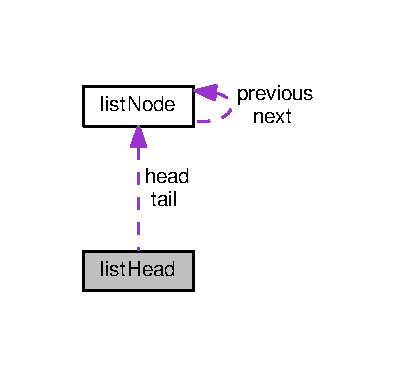
\includegraphics[width=173pt]{structlistHead__coll__graph}
\end{center}
\end{figure}
\subsection*{Public Attributes}
\begin{DoxyCompactItemize}
\item 
\mbox{\Hypertarget{structlistHead_a824ef0b95a848fde5f0dc503480edb61}\label{structlistHead_a824ef0b95a848fde5f0dc503480edb61}} 
\hyperlink{structNode}{Node} $\ast$ {\bfseries head}
\item 
\mbox{\Hypertarget{structlistHead_aafa27aceb900bf0e4ebf07857a0a94f3}\label{structlistHead_aafa27aceb900bf0e4ebf07857a0a94f3}} 
\hyperlink{structNode}{Node} $\ast$ {\bfseries tail}
\item 
\mbox{\Hypertarget{structlistHead_ae6fd9f56c9b85bd823c1c2e104c6ccaf}\label{structlistHead_ae6fd9f56c9b85bd823c1c2e104c6ccaf}} 
void($\ast$ {\bfseries delete\+Data} )(void $\ast$to\+Be\+Deleted)
\item 
\mbox{\Hypertarget{structlistHead_a0b7a3598d7dc73526fddff45a3e29595}\label{structlistHead_a0b7a3598d7dc73526fddff45a3e29595}} 
int($\ast$ {\bfseries compare} )(const void $\ast$first, const void $\ast$second)
\item 
\mbox{\Hypertarget{structlistHead_a8247a7a84929fe9e4bdac0fb8dbf4633}\label{structlistHead_a8247a7a84929fe9e4bdac0fb8dbf4633}} 
void($\ast$ {\bfseries print\+Data} )(void $\ast$to\+Be\+Printed)
\end{DoxyCompactItemize}


\subsection{Detailed Description}
Dummy head of the list. Contains no actual data on it beyond a pointer to the front and end of the list. 

The documentation for this struct was generated from the following file\+:\begin{DoxyCompactItemize}
\item 
include/\hyperlink{LinkedListAPI_8h}{Linked\+List\+A\+P\+I.\+h}\end{DoxyCompactItemize}

\hypertarget{structlistNode}{}\section{list\+Node Struct Reference}
\label{structlistNode}\index{list\+Node@{list\+Node}}


{\ttfamily \#include $<$Linked\+List\+A\+P\+I.\+h$>$}



Collaboration diagram for list\+Node\+:
\nopagebreak
\begin{figure}[H]
\begin{center}
\leavevmode
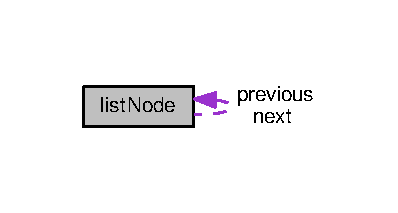
\includegraphics[width=191pt]{structlistNode__coll__graph}
\end{center}
\end{figure}
\subsection*{Public Attributes}
\begin{DoxyCompactItemize}
\item 
\mbox{\Hypertarget{structlistNode_a3d954805822577bf67d0a53a99bb337a}\label{structlistNode_a3d954805822577bf67d0a53a99bb337a}} 
void $\ast$ {\bfseries data}
\item 
\mbox{\Hypertarget{structlistNode_af4cb79db629800938019f92ce510c157}\label{structlistNode_af4cb79db629800938019f92ce510c157}} 
struct \hyperlink{structlistNode}{list\+Node} $\ast$ {\bfseries previous}
\item 
\mbox{\Hypertarget{structlistNode_a860785ea27fb1c044d6a59ba491dd6ab}\label{structlistNode_a860785ea27fb1c044d6a59ba491dd6ab}} 
struct \hyperlink{structlistNode}{list\+Node} $\ast$ {\bfseries next}
\end{DoxyCompactItemize}


\subsection{Detailed Description}
\hyperlink{structNode}{Node} of a linked list. This list is doubly linked, meaning that it has points to both the node immediately in front of it, as well as the node immediately behind it. 

The documentation for this struct was generated from the following file\+:\begin{DoxyCompactItemize}
\item 
include/\hyperlink{LinkedListAPI_8h}{Linked\+List\+A\+P\+I.\+h}\end{DoxyCompactItemize}

\hypertarget{structQueue}{}\section{Queue Struct Reference}
\label{structQueue}\index{Queue@{Queue}}


{\ttfamily \#include $<$Queue\+A\+D\+T.\+h$>$}



Collaboration diagram for Queue\+:
\nopagebreak
\begin{figure}[H]
\begin{center}
\leavevmode
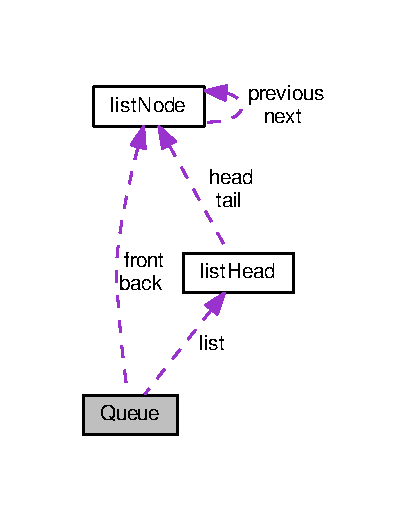
\includegraphics[width=196pt]{structQueue__coll__graph}
\end{center}
\end{figure}
\subsection*{Public Attributes}
\begin{DoxyCompactItemize}
\item 
\mbox{\Hypertarget{structQueue_a41c7eb433a01719af10cd2dc998ebdd8}\label{structQueue_a41c7eb433a01719af10cd2dc998ebdd8}} 
\hyperlink{LinkedListAPI_8h_a87906180aa2c50677fa64f2f44a25bf0}{List} $\ast$ {\bfseries list}
\item 
\mbox{\Hypertarget{structQueue_a36ab375d24d41bcc1d598c132700835b}\label{structQueue_a36ab375d24d41bcc1d598c132700835b}} 
\hyperlink{LinkedListAPI_8h_a2b677d2e8ffc156e6b24a55e7338ecad}{Node} $\ast$ {\bfseries front}
\item 
\mbox{\Hypertarget{structQueue_aaf188b8da9524a67e909f14d78563dab}\label{structQueue_aaf188b8da9524a67e909f14d78563dab}} 
\hyperlink{LinkedListAPI_8h_a2b677d2e8ffc156e6b24a55e7338ecad}{Node} $\ast$ {\bfseries back}
\item 
\mbox{\Hypertarget{structQueue_a3c0430ed080b9095895b73241ef859ac}\label{structQueue_a3c0430ed080b9095895b73241ef859ac}} 
int $\ast$ {\bfseries length}
\end{DoxyCompactItemize}


\subsection{Detailed Description}
queue structure\+: contains the list, front, back, and length of queue 

The documentation for this struct was generated from the following file\+:\begin{DoxyCompactItemize}
\item 
include/\hyperlink{QueueADT_8h}{Queue\+A\+D\+T.\+h}\end{DoxyCompactItemize}

\chapter{File Documentation}
\hypertarget{LinkedListAPI_8h}{}\section{include/\+Linked\+List\+A\+PI.h File Reference}
\label{LinkedListAPI_8h}\index{include/\+Linked\+List\+A\+P\+I.\+h@{include/\+Linked\+List\+A\+P\+I.\+h}}


File containing the function definitions of a doubly linked list.  


{\ttfamily \#include $<$stdio.\+h$>$}\newline
{\ttfamily \#include $<$stdlib.\+h$>$}\newline
Include dependency graph for Linked\+List\+A\+P\+I.\+h\+:
\nopagebreak
\begin{figure}[H]
\begin{center}
\leavevmode
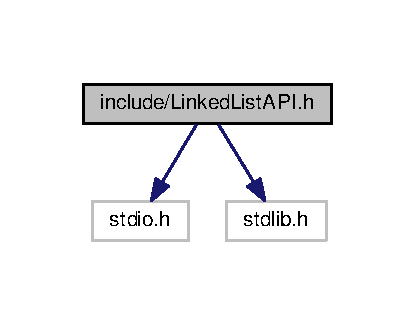
\includegraphics[width=199pt]{LinkedListAPI_8h__incl}
\end{center}
\end{figure}
This graph shows which files directly or indirectly include this file\+:
\nopagebreak
\begin{figure}[H]
\begin{center}
\leavevmode
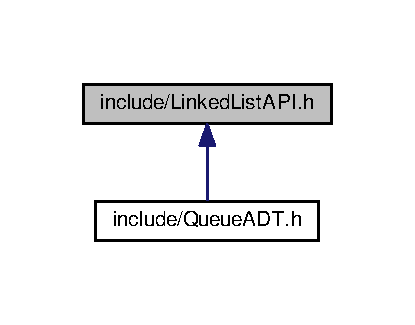
\includegraphics[width=199pt]{LinkedListAPI_8h__dep__incl}
\end{center}
\end{figure}
\subsection*{Classes}
\begin{DoxyCompactItemize}
\item 
struct \hyperlink{structlistNode}{list\+Node}
\item 
struct \hyperlink{structlistHead}{list\+Head}
\end{DoxyCompactItemize}
\subsection*{Typedefs}
\begin{DoxyCompactItemize}
\item 
typedef struct \hyperlink{structlistNode}{list\+Node} \hyperlink{LinkedListAPI_8h_a2b677d2e8ffc156e6b24a55e7338ecad}{Node}
\item 
typedef struct \hyperlink{structlistHead}{list\+Head} \hyperlink{LinkedListAPI_8h_a87906180aa2c50677fa64f2f44a25bf0}{List}
\end{DoxyCompactItemize}
\subsection*{Functions}
\begin{DoxyCompactItemize}
\item 
\hyperlink{LinkedListAPI_8h_a87906180aa2c50677fa64f2f44a25bf0}{List} $\ast$ \hyperlink{LinkedListAPI_8h_a62add6a4e99f0dff291983429bc723ef}{initialize\+List} (void($\ast$print\+Function)(void $\ast$to\+Be\+Printed), void($\ast$delete\+Function)(void $\ast$to\+Be\+Deleted), int($\ast$compare\+Function)(const void $\ast$first, const void $\ast$second))
\item 
\hyperlink{LinkedListAPI_8h_a2b677d2e8ffc156e6b24a55e7338ecad}{Node} $\ast$ \hyperlink{LinkedListAPI_8h_a1f97560bb77496690b9bb600c9d793ee}{initialize\+Node} (void $\ast$data)
\item 
void \hyperlink{LinkedListAPI_8h_a2ee6d31ae2c69ed0c7952be1f5633ba8}{insert\+Front} (\hyperlink{LinkedListAPI_8h_a87906180aa2c50677fa64f2f44a25bf0}{List} $\ast$list, void $\ast$to\+Be\+Added)
\item 
void \hyperlink{LinkedListAPI_8h_afd96360bb8bc96b5be7e2c5bf00d6bee}{insert\+Back} (\hyperlink{LinkedListAPI_8h_a87906180aa2c50677fa64f2f44a25bf0}{List} $\ast$list, void $\ast$to\+Be\+Added)
\item 
void \hyperlink{LinkedListAPI_8h_abc18ab05ec8bd1b4ea085d5b30baf536}{delete\+List} (\hyperlink{LinkedListAPI_8h_a87906180aa2c50677fa64f2f44a25bf0}{List} $\ast$list)
\item 
void \hyperlink{LinkedListAPI_8h_a34497de4d0db0b37b4e8683256f41b75}{insert\+Sorted} (\hyperlink{LinkedListAPI_8h_a87906180aa2c50677fa64f2f44a25bf0}{List} $\ast$list, void $\ast$to\+Be\+Added)
\item 
int \hyperlink{LinkedListAPI_8h_ae1a14b22705ddc68f907e6732f4d0843}{delete\+Data\+From\+List} (\hyperlink{LinkedListAPI_8h_a87906180aa2c50677fa64f2f44a25bf0}{List} $\ast$list, void $\ast$to\+Be\+Deleted)
\item 
void $\ast$ \hyperlink{LinkedListAPI_8h_aed6180e91efc5e85ad98095b0e561d39}{get\+From\+Front} (\hyperlink{LinkedListAPI_8h_a87906180aa2c50677fa64f2f44a25bf0}{List} $\ast$list)
\item 
void $\ast$ \hyperlink{LinkedListAPI_8h_ae9e342a1ac0eaf0412c69292c684e6c3}{get\+From\+Back} (\hyperlink{LinkedListAPI_8h_a87906180aa2c50677fa64f2f44a25bf0}{List} $\ast$list)
\item 
void \hyperlink{LinkedListAPI_8h_a3f8bda02985d59886112a079d7778a04}{print\+Forward} (\hyperlink{LinkedListAPI_8h_a87906180aa2c50677fa64f2f44a25bf0}{List} $\ast$list)
\item 
void \hyperlink{LinkedListAPI_8h_ae31c341dbee4ea0ecf307476304a8750}{print\+Backwards} (\hyperlink{LinkedListAPI_8h_a87906180aa2c50677fa64f2f44a25bf0}{List} $\ast$list)
\end{DoxyCompactItemize}


\subsection{Detailed Description}
File containing the function definitions of a doubly linked list. 

\begin{DoxyAuthor}{Author}
Michael Ellis 
\end{DoxyAuthor}
\begin{DoxyDate}{Date}
January 2017 
\end{DoxyDate}


\subsection{Typedef Documentation}
\mbox{\Hypertarget{LinkedListAPI_8h_a87906180aa2c50677fa64f2f44a25bf0}\label{LinkedListAPI_8h_a87906180aa2c50677fa64f2f44a25bf0}} 
\index{Linked\+List\+A\+P\+I.\+h@{Linked\+List\+A\+P\+I.\+h}!List@{List}}
\index{List@{List}!Linked\+List\+A\+P\+I.\+h@{Linked\+List\+A\+P\+I.\+h}}
\subsubsection{\texorpdfstring{List}{List}}
{\footnotesize\ttfamily typedef struct \hyperlink{structlistHead}{list\+Head}  \hyperlink{LinkedListAPI_8h_a87906180aa2c50677fa64f2f44a25bf0}{List}}

Dummy head of the list. Contains no actual data on it beyond a pointer to the front and end of the list. \mbox{\Hypertarget{LinkedListAPI_8h_a2b677d2e8ffc156e6b24a55e7338ecad}\label{LinkedListAPI_8h_a2b677d2e8ffc156e6b24a55e7338ecad}} 
\index{Linked\+List\+A\+P\+I.\+h@{Linked\+List\+A\+P\+I.\+h}!Node@{Node}}
\index{Node@{Node}!Linked\+List\+A\+P\+I.\+h@{Linked\+List\+A\+P\+I.\+h}}
\subsubsection{\texorpdfstring{Node}{Node}}
{\footnotesize\ttfamily typedef struct \hyperlink{structlistNode}{list\+Node}  \hyperlink{LinkedListAPI_8h_a2b677d2e8ffc156e6b24a55e7338ecad}{Node}}

Node of a linked list. This list is doubly linked, meaning that it has points to both the node immediately in front of it, as well as the node immediately behind it. 

\subsection{Function Documentation}
\mbox{\Hypertarget{LinkedListAPI_8h_ae1a14b22705ddc68f907e6732f4d0843}\label{LinkedListAPI_8h_ae1a14b22705ddc68f907e6732f4d0843}} 
\index{Linked\+List\+A\+P\+I.\+h@{Linked\+List\+A\+P\+I.\+h}!delete\+Data\+From\+List@{delete\+Data\+From\+List}}
\index{delete\+Data\+From\+List@{delete\+Data\+From\+List}!Linked\+List\+A\+P\+I.\+h@{Linked\+List\+A\+P\+I.\+h}}
\subsubsection{\texorpdfstring{delete\+Data\+From\+List()}{deleteDataFromList()}}
{\footnotesize\ttfamily int delete\+Data\+From\+List (\begin{DoxyParamCaption}\item[{\hyperlink{LinkedListAPI_8h_a87906180aa2c50677fa64f2f44a25bf0}{List} $\ast$}]{list,  }\item[{void $\ast$}]{to\+Be\+Deleted }\end{DoxyParamCaption})}

Function to remove a node from the list and alter the pointers accordingly to not disrupt the order of the data structure. \begin{DoxyPrecond}{Precondition}
List must exist and have memory allocated to it 
\end{DoxyPrecond}
\begin{DoxyPostcond}{Postcondition}
to\+Be\+Deleted will have its memory freed if it exists in the list. 
\end{DoxyPostcond}

\begin{DoxyParams}{Parameters}
{\em list} & pointer to the dummy head of the list containing delete\+Function function pointer \\
\hline
{\em to\+Be\+Deleted} & pointer to data that is to be removed from the list \\
\hline
\end{DoxyParams}
\begin{DoxyReturn}{Returns}
returns E\+X\+I\+T\+\_\+\+S\+U\+C\+C\+E\+SS on success, and E\+X\+I\+T\+\_\+\+F\+A\+I\+L\+U\+RE when empty. Returns -\/1 when the node cannot be found. 
\end{DoxyReturn}
\mbox{\Hypertarget{LinkedListAPI_8h_abc18ab05ec8bd1b4ea085d5b30baf536}\label{LinkedListAPI_8h_abc18ab05ec8bd1b4ea085d5b30baf536}} 
\index{Linked\+List\+A\+P\+I.\+h@{Linked\+List\+A\+P\+I.\+h}!delete\+List@{delete\+List}}
\index{delete\+List@{delete\+List}!Linked\+List\+A\+P\+I.\+h@{Linked\+List\+A\+P\+I.\+h}}
\subsubsection{\texorpdfstring{delete\+List()}{deleteList()}}
{\footnotesize\ttfamily void delete\+List (\begin{DoxyParamCaption}\item[{\hyperlink{LinkedListAPI_8h_a87906180aa2c50677fa64f2f44a25bf0}{List} $\ast$}]{list }\end{DoxyParamCaption})}

Deletes the entire linked list head to tail, starting with the nodes, followed by the list itself. \begin{DoxyPrecond}{Precondition}
\textquotesingle{}List\textquotesingle{} type must exist and be used in order to keep track of the linked list. 
\end{DoxyPrecond}

\begin{DoxyParams}{Parameters}
{\em list} & pointer to the List-\/type dummy node \\
\hline
\end{DoxyParams}
\mbox{\Hypertarget{LinkedListAPI_8h_ae9e342a1ac0eaf0412c69292c684e6c3}\label{LinkedListAPI_8h_ae9e342a1ac0eaf0412c69292c684e6c3}} 
\index{Linked\+List\+A\+P\+I.\+h@{Linked\+List\+A\+P\+I.\+h}!get\+From\+Back@{get\+From\+Back}}
\index{get\+From\+Back@{get\+From\+Back}!Linked\+List\+A\+P\+I.\+h@{Linked\+List\+A\+P\+I.\+h}}
\subsubsection{\texorpdfstring{get\+From\+Back()}{getFromBack()}}
{\footnotesize\ttfamily void$\ast$ get\+From\+Back (\begin{DoxyParamCaption}\item[{\hyperlink{LinkedListAPI_8h_a87906180aa2c50677fa64f2f44a25bf0}{List} $\ast$}]{list }\end{DoxyParamCaption})}

Function to return the data at the back of the list. \begin{DoxyPrecond}{Precondition}
The list exists and has memory allocated to it 
\end{DoxyPrecond}

\begin{DoxyParams}{Parameters}
{\em list} & pointer to the dummy head of the list containing the tail of the list \\
\hline
\end{DoxyParams}
\begin{DoxyReturn}{Returns}
pointer to the data located at the tail of the list 
\end{DoxyReturn}
\mbox{\Hypertarget{LinkedListAPI_8h_aed6180e91efc5e85ad98095b0e561d39}\label{LinkedListAPI_8h_aed6180e91efc5e85ad98095b0e561d39}} 
\index{Linked\+List\+A\+P\+I.\+h@{Linked\+List\+A\+P\+I.\+h}!get\+From\+Front@{get\+From\+Front}}
\index{get\+From\+Front@{get\+From\+Front}!Linked\+List\+A\+P\+I.\+h@{Linked\+List\+A\+P\+I.\+h}}
\subsubsection{\texorpdfstring{get\+From\+Front()}{getFromFront()}}
{\footnotesize\ttfamily void$\ast$ get\+From\+Front (\begin{DoxyParamCaption}\item[{\hyperlink{LinkedListAPI_8h_a87906180aa2c50677fa64f2f44a25bf0}{List} $\ast$}]{list }\end{DoxyParamCaption})}

Function to return the data at the front of the list. \begin{DoxyPrecond}{Precondition}
The list exists and has memory allocated to it 
\end{DoxyPrecond}

\begin{DoxyParams}{Parameters}
{\em list} & pointer to the dummy head of the list containing the head of the list \\
\hline
\end{DoxyParams}
\begin{DoxyReturn}{Returns}
pointer to the data located at the head of the list 
\end{DoxyReturn}
\mbox{\Hypertarget{LinkedListAPI_8h_a62add6a4e99f0dff291983429bc723ef}\label{LinkedListAPI_8h_a62add6a4e99f0dff291983429bc723ef}} 
\index{Linked\+List\+A\+P\+I.\+h@{Linked\+List\+A\+P\+I.\+h}!initialize\+List@{initialize\+List}}
\index{initialize\+List@{initialize\+List}!Linked\+List\+A\+P\+I.\+h@{Linked\+List\+A\+P\+I.\+h}}
\subsubsection{\texorpdfstring{initialize\+List()}{initializeList()}}
{\footnotesize\ttfamily \hyperlink{LinkedListAPI_8h_a87906180aa2c50677fa64f2f44a25bf0}{List}$\ast$ initialize\+List (\begin{DoxyParamCaption}\item[{void($\ast$)(void $\ast$to\+Be\+Printed)}]{print\+Function,  }\item[{void($\ast$)(void $\ast$to\+Be\+Deleted)}]{delete\+Function,  }\item[{int($\ast$)(const void $\ast$first, const void $\ast$second)}]{compare\+Function }\end{DoxyParamCaption})}

Function to point the list head to the appropriate functions. Allocates memory to the struct. \begin{DoxyReturn}{Returns}
pointer to the list head 
\end{DoxyReturn}

\begin{DoxyParams}{Parameters}
{\em print\+Function} & function pointer to print a single node of the list \\
\hline
{\em delete\+Function} & function pointer to delete a single piece of data from the list \\
\hline
{\em compare\+Function} & function pointer to compare two nodes of the list in order to test for equality or order \\
\hline
\end{DoxyParams}
\mbox{\Hypertarget{LinkedListAPI_8h_a1f97560bb77496690b9bb600c9d793ee}\label{LinkedListAPI_8h_a1f97560bb77496690b9bb600c9d793ee}} 
\index{Linked\+List\+A\+P\+I.\+h@{Linked\+List\+A\+P\+I.\+h}!initialize\+Node@{initialize\+Node}}
\index{initialize\+Node@{initialize\+Node}!Linked\+List\+A\+P\+I.\+h@{Linked\+List\+A\+P\+I.\+h}}
\subsubsection{\texorpdfstring{initialize\+Node()}{initializeNode()}}
{\footnotesize\ttfamily \hyperlink{LinkedListAPI_8h_a2b677d2e8ffc156e6b24a55e7338ecad}{Node}$\ast$ initialize\+Node (\begin{DoxyParamCaption}\item[{void $\ast$}]{data }\end{DoxyParamCaption})}

Function for creating a node for a linked list. This node contains generic data and may be connected to other notes in a list. \begin{DoxyPrecond}{Precondition}
data should be of same size of void pointer on the users machine to avoid size conflicts. data must be valid. data must be cast to void pointer before being added. 
\end{DoxyPrecond}
\begin{DoxyPostcond}{Postcondition}
data is valid to be added to a linked list 
\end{DoxyPostcond}
\begin{DoxyReturn}{Returns}
On success returns a node that can be added to a linked list. On failure, returns N\+U\+LL. 
\end{DoxyReturn}

\begin{DoxyParams}{Parameters}
{\em data} & -\/ is a generic pointer to any data type. \\
\hline
\end{DoxyParams}
\mbox{\Hypertarget{LinkedListAPI_8h_afd96360bb8bc96b5be7e2c5bf00d6bee}\label{LinkedListAPI_8h_afd96360bb8bc96b5be7e2c5bf00d6bee}} 
\index{Linked\+List\+A\+P\+I.\+h@{Linked\+List\+A\+P\+I.\+h}!insert\+Back@{insert\+Back}}
\index{insert\+Back@{insert\+Back}!Linked\+List\+A\+P\+I.\+h@{Linked\+List\+A\+P\+I.\+h}}
\subsubsection{\texorpdfstring{insert\+Back()}{insertBack()}}
{\footnotesize\ttfamily void insert\+Back (\begin{DoxyParamCaption}\item[{\hyperlink{LinkedListAPI_8h_a87906180aa2c50677fa64f2f44a25bf0}{List} $\ast$}]{list,  }\item[{void $\ast$}]{to\+Be\+Added }\end{DoxyParamCaption})}

Inserts a Node to the back of a linked list. The list then updates accordingly to adhere to the A\+DT. \begin{DoxyPrecond}{Precondition}
\textquotesingle{}List\textquotesingle{} type must exist and be used in order to keep track of the linked list. 
\end{DoxyPrecond}

\begin{DoxyParams}{Parameters}
{\em list} & pointer to the dummy head of the list \\
\hline
{\em to\+Be\+Added} & a pointer to data that is to be added to the linked list \\
\hline
\end{DoxyParams}
\mbox{\Hypertarget{LinkedListAPI_8h_a2ee6d31ae2c69ed0c7952be1f5633ba8}\label{LinkedListAPI_8h_a2ee6d31ae2c69ed0c7952be1f5633ba8}} 
\index{Linked\+List\+A\+P\+I.\+h@{Linked\+List\+A\+P\+I.\+h}!insert\+Front@{insert\+Front}}
\index{insert\+Front@{insert\+Front}!Linked\+List\+A\+P\+I.\+h@{Linked\+List\+A\+P\+I.\+h}}
\subsubsection{\texorpdfstring{insert\+Front()}{insertFront()}}
{\footnotesize\ttfamily void insert\+Front (\begin{DoxyParamCaption}\item[{\hyperlink{LinkedListAPI_8h_a87906180aa2c50677fa64f2f44a25bf0}{List} $\ast$}]{list,  }\item[{void $\ast$}]{to\+Be\+Added }\end{DoxyParamCaption})}

Inserts a Node to the front of a linked list. The list then updates accordingly to adhere to the A\+DT. \begin{DoxyPrecond}{Precondition}
\textquotesingle{}List\textquotesingle{} type must exist and be used in order to keep track of the linked list. 
\end{DoxyPrecond}

\begin{DoxyParams}{Parameters}
{\em list} & pointer to the dummy head of the list \\
\hline
{\em to\+Be\+Added} & a pointer to data that is to be added to the linked list \\
\hline
\end{DoxyParams}
\mbox{\Hypertarget{LinkedListAPI_8h_a34497de4d0db0b37b4e8683256f41b75}\label{LinkedListAPI_8h_a34497de4d0db0b37b4e8683256f41b75}} 
\index{Linked\+List\+A\+P\+I.\+h@{Linked\+List\+A\+P\+I.\+h}!insert\+Sorted@{insert\+Sorted}}
\index{insert\+Sorted@{insert\+Sorted}!Linked\+List\+A\+P\+I.\+h@{Linked\+List\+A\+P\+I.\+h}}
\subsubsection{\texorpdfstring{insert\+Sorted()}{insertSorted()}}
{\footnotesize\ttfamily void insert\+Sorted (\begin{DoxyParamCaption}\item[{\hyperlink{LinkedListAPI_8h_a87906180aa2c50677fa64f2f44a25bf0}{List} $\ast$}]{list,  }\item[{void $\ast$}]{to\+Be\+Added }\end{DoxyParamCaption})}

Uses the comparison function in the List struct to place the element in the appropriate position in the list. this is intended to be used from the beginning in order to keep the list completely sorted. \begin{DoxyPrecond}{Precondition}
List exists and has memory allocated to it. Node to be added is valid. 
\end{DoxyPrecond}
\begin{DoxyPostcond}{Postcondition}
The node to be added will be placed immediately before or after the first occurrence of a related node 
\end{DoxyPostcond}

\begin{DoxyParams}{Parameters}
{\em list} & a pointer to the dummy head of the list containing function pointers for delete and compare, as well as a pointer to the first and last element of the list. \\
\hline
{\em to\+Be\+Added} & a pointer to data that is to be added to the linked list \\
\hline
\end{DoxyParams}
\mbox{\Hypertarget{LinkedListAPI_8h_ae31c341dbee4ea0ecf307476304a8750}\label{LinkedListAPI_8h_ae31c341dbee4ea0ecf307476304a8750}} 
\index{Linked\+List\+A\+P\+I.\+h@{Linked\+List\+A\+P\+I.\+h}!print\+Backwards@{print\+Backwards}}
\index{print\+Backwards@{print\+Backwards}!Linked\+List\+A\+P\+I.\+h@{Linked\+List\+A\+P\+I.\+h}}
\subsubsection{\texorpdfstring{print\+Backwards()}{printBackwards()}}
{\footnotesize\ttfamily void print\+Backwards (\begin{DoxyParamCaption}\item[{\hyperlink{LinkedListAPI_8h_a87906180aa2c50677fa64f2f44a25bf0}{List} $\ast$}]{list }\end{DoxyParamCaption})}

Function to print list from tail to head. This will utilize the list\textquotesingle{}s print\+Data function pointer to print. \begin{DoxyPrecond}{Precondition}
List must exist, but does not have to have elements. 
\end{DoxyPrecond}

\begin{DoxyParams}{Parameters}
{\em list} & Pointer to linked list dummy head. \\
\hline
\end{DoxyParams}
\mbox{\Hypertarget{LinkedListAPI_8h_a3f8bda02985d59886112a079d7778a04}\label{LinkedListAPI_8h_a3f8bda02985d59886112a079d7778a04}} 
\index{Linked\+List\+A\+P\+I.\+h@{Linked\+List\+A\+P\+I.\+h}!print\+Forward@{print\+Forward}}
\index{print\+Forward@{print\+Forward}!Linked\+List\+A\+P\+I.\+h@{Linked\+List\+A\+P\+I.\+h}}
\subsubsection{\texorpdfstring{print\+Forward()}{printForward()}}
{\footnotesize\ttfamily void print\+Forward (\begin{DoxyParamCaption}\item[{\hyperlink{LinkedListAPI_8h_a87906180aa2c50677fa64f2f44a25bf0}{List} $\ast$}]{list }\end{DoxyParamCaption})}

Function to print list from head to tail. This will utilize the list\textquotesingle{}s print\+Data function pointer to print. \begin{DoxyPrecond}{Precondition}
List must exist, but does not have to have elements. 
\end{DoxyPrecond}

\begin{DoxyParams}{Parameters}
{\em list} & Pointer to linked list dummy head. \\
\hline
\end{DoxyParams}

\hypertarget{QueueADT_8h}{}\section{include/\+Queue\+A\+DT.h File Reference}
\label{QueueADT_8h}\index{include/\+Queue\+A\+D\+T.\+h@{include/\+Queue\+A\+D\+T.\+h}}


File containing the function definitions of a queue.  


{\ttfamily \#include $<$stdio.\+h$>$}\newline
{\ttfamily \#include $<$stdbool.\+h$>$}\newline
{\ttfamily \#include \char`\"{}Linked\+List\+A\+P\+I.\+h\char`\"{}}\newline
Include dependency graph for Queue\+A\+D\+T.\+h\+:
\nopagebreak
\begin{figure}[H]
\begin{center}
\leavevmode
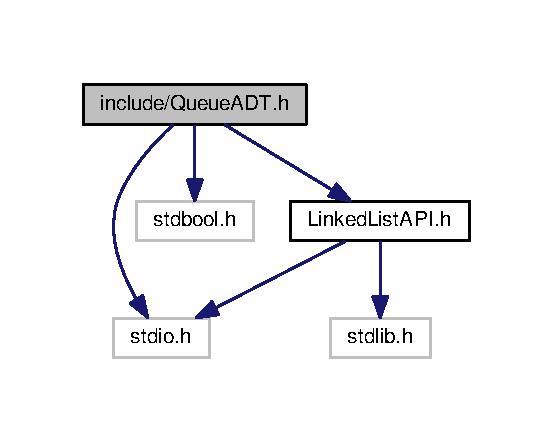
\includegraphics[width=266pt]{QueueADT_8h__incl}
\end{center}
\end{figure}
\subsection*{Classes}
\begin{DoxyCompactItemize}
\item 
struct \hyperlink{structQueue}{Queue}
\item 
struct \hyperlink{structcar}{car}
\end{DoxyCompactItemize}
\subsection*{Typedefs}
\begin{DoxyCompactItemize}
\item 
typedef struct \hyperlink{structQueue}{Queue} \hyperlink{QueueADT_8h_ad4f29a362a072ba563b41ae8e935c6fc}{Queue}
\item 
typedef struct \hyperlink{structcar}{car} \hyperlink{QueueADT_8h_a17808c9c3518e92cb43835e3bfa9f878}{car}
\end{DoxyCompactItemize}
\subsection*{Functions}
\begin{DoxyCompactItemize}
\item 
\hyperlink{structQueue}{Queue} $\ast$ \hyperlink{QueueADT_8h_accc2c49d11d601a77eb598c3741ffe9a}{create} ()
\item 
void \hyperlink{QueueADT_8h_a89893c23833b9fa8e7dde90343ca8885}{destroy} (\hyperlink{structQueue}{Queue} $\ast$p\+Queue)
\item 
void \hyperlink{QueueADT_8h_a719e32872e4862e2cd83281e87b60ed1}{enqueue} (\hyperlink{structQueue}{Queue} $\ast$p\+Queue, void $\ast$data)
\item 
void $\ast$ \hyperlink{QueueADT_8h_a045ef43f63919ca19115c060344cdac0}{dequeue} (\hyperlink{structQueue}{Queue} $\ast$p\+Queue)
\item 
void $\ast$ \hyperlink{QueueADT_8h_a8fa514a5fd902bd2fe46d57d14d1ae8a}{peek} (\hyperlink{structQueue}{Queue} $\ast$p\+Queue)
\item 
bool \hyperlink{QueueADT_8h_ae28fcf858ea1c33ed0b56eb82b647306}{is\+Empty} (\hyperlink{structQueue}{Queue} $\ast$p\+Queue)
\item 
int \hyperlink{QueueADT_8h_ab6692939eeb89d044d92061a6501e505}{compare} (const void $\ast$first, const void $\ast$second)
\end{DoxyCompactItemize}


\subsection{Detailed Description}
File containing the function definitions of a queue. 

\begin{DoxyAuthor}{Author}
Braelyn Rotman 
\end{DoxyAuthor}
\begin{DoxyDate}{Date}
June 2, 2018 
\end{DoxyDate}


\subsection{Typedef Documentation}
\mbox{\Hypertarget{QueueADT_8h_a17808c9c3518e92cb43835e3bfa9f878}\label{QueueADT_8h_a17808c9c3518e92cb43835e3bfa9f878}} 
\index{Queue\+A\+D\+T.\+h@{Queue\+A\+D\+T.\+h}!car@{car}}
\index{car@{car}!Queue\+A\+D\+T.\+h@{Queue\+A\+D\+T.\+h}}
\subsubsection{\texorpdfstring{car}{car}}
{\footnotesize\ttfamily typedef struct \hyperlink{structcar}{car} \hyperlink{structcar}{car}}

car structure\+: this is the data that will be stored in the queue \mbox{\Hypertarget{QueueADT_8h_ad4f29a362a072ba563b41ae8e935c6fc}\label{QueueADT_8h_ad4f29a362a072ba563b41ae8e935c6fc}} 
\index{Queue\+A\+D\+T.\+h@{Queue\+A\+D\+T.\+h}!Queue@{Queue}}
\index{Queue@{Queue}!Queue\+A\+D\+T.\+h@{Queue\+A\+D\+T.\+h}}
\subsubsection{\texorpdfstring{Queue}{Queue}}
{\footnotesize\ttfamily typedef struct \hyperlink{structQueue}{Queue} \hyperlink{structQueue}{Queue}}

queue structure\+: contains the list, front, back, and length of queue 

\subsection{Function Documentation}
\mbox{\Hypertarget{QueueADT_8h_ab6692939eeb89d044d92061a6501e505}\label{QueueADT_8h_ab6692939eeb89d044d92061a6501e505}} 
\index{Queue\+A\+D\+T.\+h@{Queue\+A\+D\+T.\+h}!compare@{compare}}
\index{compare@{compare}!Queue\+A\+D\+T.\+h@{Queue\+A\+D\+T.\+h}}
\subsubsection{\texorpdfstring{compare()}{compare()}}
{\footnotesize\ttfamily int compare (\begin{DoxyParamCaption}\item[{const void $\ast$}]{first,  }\item[{const void $\ast$}]{second }\end{DoxyParamCaption})}

Function to compare two elements 
\begin{DoxyParams}{Parameters}
{\em first} & const void data \\
\hline
{\em second} & const void data \\
\hline
\end{DoxyParams}
\begin{DoxyReturn}{Returns}
-\/1 if first is smaller, 0 if equal, 1 if first is larger 
\end{DoxyReturn}
\mbox{\Hypertarget{QueueADT_8h_accc2c49d11d601a77eb598c3741ffe9a}\label{QueueADT_8h_accc2c49d11d601a77eb598c3741ffe9a}} 
\index{Queue\+A\+D\+T.\+h@{Queue\+A\+D\+T.\+h}!create@{create}}
\index{create@{create}!Queue\+A\+D\+T.\+h@{Queue\+A\+D\+T.\+h}}
\subsubsection{\texorpdfstring{create()}{create()}}
{\footnotesize\ttfamily \hyperlink{structQueue}{Queue}$\ast$ create (\begin{DoxyParamCaption}{ }\end{DoxyParamCaption})}

Creates and Initializes a queue. Allocates memory to the struct. \begin{DoxyReturn}{Returns}
pointer to the queue 
\end{DoxyReturn}
\mbox{\Hypertarget{QueueADT_8h_a045ef43f63919ca19115c060344cdac0}\label{QueueADT_8h_a045ef43f63919ca19115c060344cdac0}} 
\index{Queue\+A\+D\+T.\+h@{Queue\+A\+D\+T.\+h}!dequeue@{dequeue}}
\index{dequeue@{dequeue}!Queue\+A\+D\+T.\+h@{Queue\+A\+D\+T.\+h}}
\subsubsection{\texorpdfstring{dequeue()}{dequeue()}}
{\footnotesize\ttfamily void$\ast$ dequeue (\begin{DoxyParamCaption}\item[{\hyperlink{structQueue}{Queue} $\ast$}]{p\+Queue }\end{DoxyParamCaption})}

Function removed a Node from the front of a queue. \begin{DoxyPrecond}{Precondition}
\textquotesingle{}\hyperlink{structQueue}{Queue}\textquotesingle{} type must exist and not be empty 
\end{DoxyPrecond}

\begin{DoxyParams}{Parameters}
{\em p\+Queue} & pointer to the queue \\
\hline
\end{DoxyParams}
\begin{DoxyReturn}{Returns}
the removed element 
\end{DoxyReturn}
\mbox{\Hypertarget{QueueADT_8h_a89893c23833b9fa8e7dde90343ca8885}\label{QueueADT_8h_a89893c23833b9fa8e7dde90343ca8885}} 
\index{Queue\+A\+D\+T.\+h@{Queue\+A\+D\+T.\+h}!destroy@{destroy}}
\index{destroy@{destroy}!Queue\+A\+D\+T.\+h@{Queue\+A\+D\+T.\+h}}
\subsubsection{\texorpdfstring{destroy()}{destroy()}}
{\footnotesize\ttfamily void destroy (\begin{DoxyParamCaption}\item[{\hyperlink{structQueue}{Queue} $\ast$}]{p\+Queue }\end{DoxyParamCaption})}

Function to delete all data within the queue \begin{DoxyPrecond}{Precondition}
\textquotesingle{}\hyperlink{structQueue}{Queue}\textquotesingle{} type must exist 
\end{DoxyPrecond}

\begin{DoxyParams}{Parameters}
{\em p\+Queue} & pointer to the queue to destroy \\
\hline
\end{DoxyParams}
\mbox{\Hypertarget{QueueADT_8h_a719e32872e4862e2cd83281e87b60ed1}\label{QueueADT_8h_a719e32872e4862e2cd83281e87b60ed1}} 
\index{Queue\+A\+D\+T.\+h@{Queue\+A\+D\+T.\+h}!enqueue@{enqueue}}
\index{enqueue@{enqueue}!Queue\+A\+D\+T.\+h@{Queue\+A\+D\+T.\+h}}
\subsubsection{\texorpdfstring{enqueue()}{enqueue()}}
{\footnotesize\ttfamily void enqueue (\begin{DoxyParamCaption}\item[{\hyperlink{structQueue}{Queue} $\ast$}]{p\+Queue,  }\item[{void $\ast$}]{data }\end{DoxyParamCaption})}

Fucntion inserts a Node to the back of a queue. \begin{DoxyPrecond}{Precondition}
\textquotesingle{}\hyperlink{structQueue}{Queue}\textquotesingle{} type must exist 
\end{DoxyPrecond}

\begin{DoxyParams}{Parameters}
{\em p\+Queue} & pointer to the queue \\
\hline
{\em data} & a pointer to data that is to be added to the queue \\
\hline
\end{DoxyParams}
\mbox{\Hypertarget{QueueADT_8h_ae28fcf858ea1c33ed0b56eb82b647306}\label{QueueADT_8h_ae28fcf858ea1c33ed0b56eb82b647306}} 
\index{Queue\+A\+D\+T.\+h@{Queue\+A\+D\+T.\+h}!is\+Empty@{is\+Empty}}
\index{is\+Empty@{is\+Empty}!Queue\+A\+D\+T.\+h@{Queue\+A\+D\+T.\+h}}
\subsubsection{\texorpdfstring{is\+Empty()}{isEmpty()}}
{\footnotesize\ttfamily bool is\+Empty (\begin{DoxyParamCaption}\item[{\hyperlink{structQueue}{Queue} $\ast$}]{p\+Queue }\end{DoxyParamCaption})}

Function to check if a queue is empty. \begin{DoxyPrecond}{Precondition}
\textquotesingle{}\hyperlink{structQueue}{Queue}\textquotesingle{} type must exist 
\end{DoxyPrecond}

\begin{DoxyParams}{Parameters}
{\em p\+Queue} & pointer to the queue \\
\hline
\end{DoxyParams}
\begin{DoxyReturn}{Returns}
true if empty or false if not 
\end{DoxyReturn}
\mbox{\Hypertarget{QueueADT_8h_a8fa514a5fd902bd2fe46d57d14d1ae8a}\label{QueueADT_8h_a8fa514a5fd902bd2fe46d57d14d1ae8a}} 
\index{Queue\+A\+D\+T.\+h@{Queue\+A\+D\+T.\+h}!peek@{peek}}
\index{peek@{peek}!Queue\+A\+D\+T.\+h@{Queue\+A\+D\+T.\+h}}
\subsubsection{\texorpdfstring{peek()}{peek()}}
{\footnotesize\ttfamily void$\ast$ peek (\begin{DoxyParamCaption}\item[{\hyperlink{structQueue}{Queue} $\ast$}]{p\+Queue }\end{DoxyParamCaption})}

Function to look at the front of a queue without removing it. \begin{DoxyPrecond}{Precondition}
\textquotesingle{}\hyperlink{structQueue}{Queue}\textquotesingle{} type must exist and be initialized 
\end{DoxyPrecond}

\begin{DoxyParams}{Parameters}
{\em p\+Queue} & pointer to the queue \\
\hline
\end{DoxyParams}
\begin{DoxyReturn}{Returns}
the first element in the queue 
\end{DoxyReturn}

%--- End generated contents ---

% Index
\backmatter
\newpage
\phantomsection
\clearemptydoublepage
\addcontentsline{toc}{chapter}{Index}
\printindex

\end{document}
